
% \iffalse
\let\negmedspace\undefined
\let\negthickspace\undefined
\documentclass[journal,12pt,twocolumn]{IEEEtran}
\usepackage{cite}
\usepackage{amsmath,amssymb,amsfonts,amsthm}
\usepackage{algorithmic}
\usepackage{graphicx}
\usepackage{textcomp}
\usepackage{xcolor}
\usepackage{txfonts}
\usepackage{listings}
\usepackage{enumitem}
\usepackage{mathtools}
\usepackage{gensymb}
\usepackage{comment}
\usepackage[breaklinks=true]{hyperref}
\usepackage{tkz-euclide} 
\usepackage{listings}
\usepackage{gvv}                                        
\def\inputGnumericTable{}                                
\usepackage[latin1]{inputenc}                            
\usepackage{color}                                       
\usepackage{array}                                       
\usepackage{longtable}                                   
\usepackage{calc}                                        
\usepackage{multirow}                                    
\usepackage{hhline}                                      
\usepackage{ifthen}                                      
\usepackage{lscape}
\usepackage{amsmath}
\newtheorem{theorem}{Theorem}[section]
\newtheorem{problem}{Problem}
\newtheorem{proposition}{Proposition}[section]
\newtheorem{lemma}{Lemma}[section]
\newtheorem{corollary}[theorem]{Corollary}
\newtheorem{example}{Example}[section]
\newtheorem{definition}[problem]{Definition}
\newcommand{\BEQA}{\begin{eqnarray}}
\newcommand{\EEQA}{\end{eqnarray}}
\newcommand{\define}{\stackrel{\triangle}{=}}
\theoremstyle{remark}
\newtheorem{rem}{Remark}



\usepackage{amsmath} % Include the amsmath package for align environment

\begin{document}

\bibliographystyle{IEEEtran}

\vspace{3cm}

\title{NCERT Physics Chapter-15 Q7}
\author{EE23BTECH11059 - Tejas$^{}$}
\maketitle

\newpage

\Huge \textbf{QUESTION 7:} \\

\medskip
\Large
A hospital uses an ultrasonic scanner to locate tumors in a tissue. What is the
wavelength of sound in the tissue in which the speed of sound is $1.7 \, \text{km/s}$? The operating frequency of the scanner is $4.2 \, \text{MHz}$.
\bigskip
\\
\Large
\textbf{SOLUTION:} \\
\begin{table}[h]
    \centering  
    \begin{tabular}{|c|c|c|}
        \hline
        Input Parameter & Value & Description \\
        \hline
        $c$ & $1.7\times10^3$ & Speed of Wave  \\
        \hline
        $f$ & $4.2\times10^6$ & Frequency  \\
        \hline
        $A$ & 1 & Wave Amplitude \\
        \hline
        $T$ & $2.38\times10^-7$ & Time period \\
        \hline
        $s(t)$ & $s(t)=A\cos(2\pi f t+\phi)$ & Wave equation \\
        \hline
        $\lambda$ & $\frac{c}{f}$ & Wavelength (to be found) \\
        \hline
    \end{tabular}
\end{table} 
\begin{figure}[h]
    \centering
    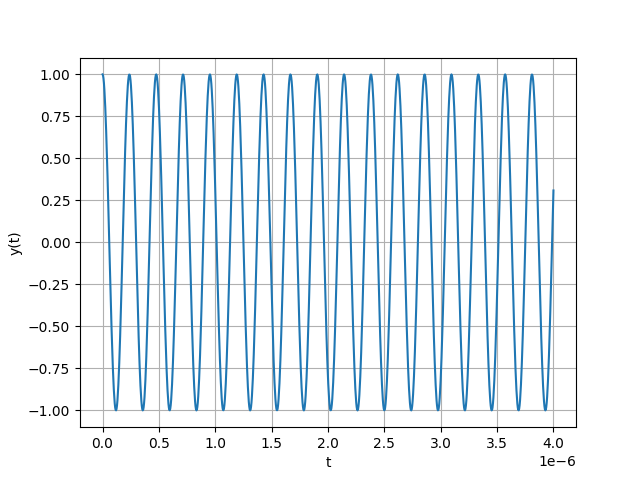
\includegraphics[width=\columnwidth]{images/plot.png}
    \caption{Waveplot}
    \label{fig:Plot1}
\end{figure}





        
        
        
             
             
        

        













\renewcommand{\thefigure}{\theenumi}
\renewcommand{\thetable}{\theenumi}





\end{document}
